% \begingroup
% \definecolor{motfill}{HTML}{F8FAFC}
% \definecolor{motborder}{HTML}{475569}
% \definecolor{motarrow}{HTML}{64748B}
% \definecolor{mottext}{HTML}{1E293B}
% \definecolor{motaccent}{HTML}{9A4A32}
% \begin{tikzpicture}[
%     >=stealth,
%     font=\sffamily\fontsize{10}{12}\selectfont,
%     box/.style={draw=motborder, fill=motfill, text=mottext,
%         line width=0.6pt, rounded corners=2pt,
%         align=center, inner xsep=8pt, inner ysep=9pt},
%     panel/.style={box, text width=5.4cm, minimum height=2.9cm},
%     flow/.style={->, draw=motarrow, line width=0.85pt,
%         shorten <=2pt, shorten >=2pt},
%     compare/.style={->, draw=motarrow, line width=0.85pt,
%         shorten <=2pt, shorten >=2pt},
%     icon/.style={draw=motborder, line width=0.8pt,
%         line cap=round, line join=round},
%     pics/person/.style={code={
%         \draw[icon] (0,0.12) circle (0.11);
%         \draw[icon] (-0.22,-0.22) .. controls (-0.22,0.02)
%             and (0.22,0.02) .. (0.22,-0.22) -- cycle;
%     }},
%     pics/record/.style={code={
%         \draw[icon] (-0.18,-0.23) rectangle (0.18,0.23);
%         \foreach \y in {-0.12,0,0.12}
%             \draw[icon] (-0.10,\y) -- (0.10,\y);
%     }},
%     pics/ai/.style={code={
%         \draw[icon,rounded corners=1pt]
%             (-0.18,-0.18) rectangle (0.18,0.18);
%         \foreach \p in {-0.09,0.09}{
%             \draw[icon] (\p,0.18) -- (\p,0.27);
%             \draw[icon] (\p,-0.18) -- (\p,-0.27);
%             \draw[icon] (0.18,\p) -- (0.27,\p);
%             \draw[icon] (-0.18,\p) -- (-0.27,\p);
%         }
%         \node[text=motborder,font=\sffamily\tiny] at (0,0) {AI};
%     }},
%     pics/mismatch/.style={code={
%         \draw[icon,draw=motaccent] (0,0) circle (0.23);
%         \draw[icon,draw=motaccent] (-0.11,0.06) -- (0.11,0.06);
%         \draw[icon,draw=motaccent] (-0.11,-0.06) -- (0.11,-0.06);
%         \draw[icon,draw=motaccent] (-0.07,-0.15) -- (0.07,0.15);
%     }},
%     pics/payment/.style={code={
%         \draw[icon,rounded corners=1pt]
%             (-0.28,-0.18) rectangle (0.28,0.18);
%         \draw[icon] (-0.28,0.05) -- (0.28,0.05);
%         \draw[icon] (-0.19,-0.09) -- (-0.04,-0.09);
%     }}
% ]
% \node[box, text width=11.9cm] (request) at (0,0)
%     {\rule{0pt}{0.48cm}\\[2pt]\textbf{Employee request}\\[4pt]
%     ``Order 100 packaging boxes from our approved supplier.''};

% \node[panel] (record) at (-3.25,-3.25)
%     {\rule{0pt}{0.48cm}\\[2pt]\textbf{Approved supplier record}\\[7pt]
%     Supplier A\\[4pt]
%     Registered account: \textbf{Account A}};

% \node[panel] (candidate) at (3.25,-3.25)
%     {\rule{0pt}{0.48cm}\\[2pt]\textbf{AI payment instruction}\\[7pt]
%     Supplier A\\[4pt]
%     Selected account: \textcolor{motaccent}{\textbf{Account B}}};

% \pic at ([yshift=-0.40cm]request.north) {person};
% \pic at ([yshift=-0.45cm]record.north) {record};
% \pic at ([yshift=-0.45cm]candidate.north) {ai};

% \draw[flow] (request.south -| record.north) -- (record.north);
% \draw[flow] (request.south -| candidate.north) -- (candidate.north);

% \node[box, draw=motaccent, text width=11.9cm] (mismatch) at (0,-6.2)
%     {\rule{0pt}{0.48cm}\\[2pt]\textbf{Account mismatch}};

% \pic at ([yshift=-0.40cm]mismatch.north) {mismatch};

% \draw[compare] (record.south) -- (record.south |- mismatch.north);
% \draw[compare] (candidate.south) -- (candidate.south |- mismatch.north);

% \node[box, text width=11.9cm] (consequence) at (0,-8.75)
%     {\rule{0pt}{0.48cm}\\[2pt]\textbf{Without verification}\\[4pt]
%     Payment may reach the wrong account.};
% \pic at ([yshift=-0.40cm]consequence.north) {payment};
% \draw[flow] (mismatch.south) -- (consequence.north);
% \end{tikzpicture}
% \endgroup

% Requires \usepackage{tikz}. Drawing only; keep the figure
% environment and its label in the introduction chapter.
\begingroup
\definecolor{motborder}{HTML}{475569}
\definecolor{motfill}{HTML}{F8FAFC}
\definecolor{mottext}{HTML}{1E293B}
\definecolor{motaccent}{HTML}{914832}

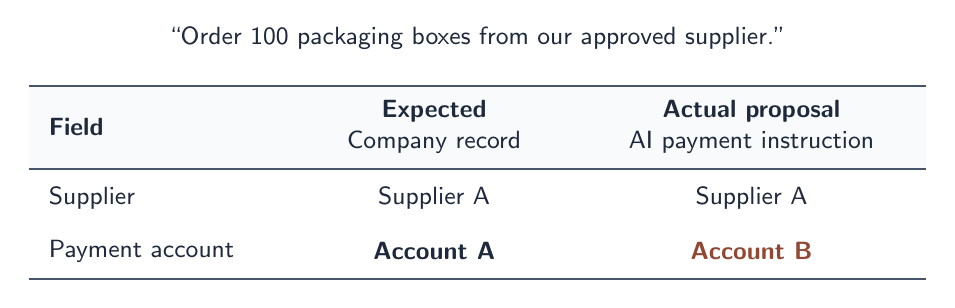
\begin{tikzpicture}[
    x=1cm, y=1cm,
    font=\sffamily\small,
    every node/.style={text=mottext, inner sep=0pt}
]
% The request provides context for both columns.
\node[align=center, text width=11.4cm] at (0,0)
    {``Order 100 packaging boxes from our approved supplier.''};

% Comparison table: fields at left, expected and proposed values at right.
\fill[motfill] (-5.7,-0.60) rectangle (5.7,-1.65);
\draw[motborder, line width=0.7pt]
    (-5.7,-0.60) -- (5.7,-0.60)
    (-5.7,-1.65) -- (5.7,-1.65)
    (-5.7,-3.05) -- (5.7,-3.05);

\node[anchor=west, font=\sffamily\small\bfseries]
    at (-5.45,-1.12) {Field};
\node[align=center] at (-0.55,-1.12)
    {\textbf{Expected}\\Company record};
\node[align=center] at (3.48,-1.12)
    {\textbf{Actual proposal}\\AI payment instruction};

\node[anchor=west] at (-5.45,-2.03) {Supplier};
\node at (-0.55,-2.03) {Supplier A};
\node at (3.48,-2.03) {Supplier A};

\node[anchor=west] at (-5.45,-2.70) {Payment account};
\node at (-0.55,-2.70) {\textbf{Account A}};
\node[text=motaccent] at (3.48,-2.70) {\textbf{Account B}};
\end{tikzpicture}
\endgroup